\documentclass[11pt]{article}

\usepackage[utf8]{inputenc}
\usepackage[T1]{fontenc}
\usepackage{lmodern}
\usepackage[protrusion=true,expansion=true]{microtype}
\usepackage{amsmath,amssymb}
\usepackage{graphicx}
\graphicspath{{figs/}}
\usepackage{booktabs}
\usepackage{array}
\usepackage[margin=1in]{geometry}
\usepackage{natbib}
\usepackage{xcolor}
\usepackage{float}
\usepackage[font=small,labelfont=bf,labelsep=period,margin=0.6cm]{caption}
\usepackage[hidelinks]{hyperref}
\hypersetup{colorlinks=true, linkcolor={black!70!blue}, citecolor={black!60!green}, urlcolor={black!70!blue}}

% --- table + spacing niceties ---
\renewcommand{\arraystretch}{1.15}
\setlength{\parskip}{0pt}
\setlength{\tabcolsep}{8pt}
\newcolumntype{L}[1]{>{\raggedright\arraybackslash}p{#1}}

\title{\bfseries A Scaffold-Disjoint QSAR Benchmark for PIM1 Kinase Inhibition\\[2pt]
\large Classical Machine-Learning Models on a Frozen ChEMBL IC$_{50}$ Dataset}

\author{Tair Narynov}

\date{\today}

\begin{document}

% Generated from the completed VM evaluation; see generate_manuscript_artifacts.py.
% Generated by generate_manuscript_artifacts.py; do not edit by hand.
\newcommand{\SelectedModel}{StackingEnsemble}
\newcommand{\SelectedCVRtwo}{0.700}
\newcommand{\SelectedCVRtwoSD}{0.015}
\newcommand{\SelectedHoldoutRtwo}{0.705}
\newcommand{\SelectedHoldoutRMSE}{0.711}
\newcommand{\SelectedHoldoutMAE}{0.542}
\newcommand{\BootstrapRtwoLower}{0.650}
\newcommand{\BootstrapRtwoUpper}{0.746}
\newcommand{\BootstrapRMSELower}{0.659}
\newcommand{\BootstrapRMSEUpper}{0.764}
\newcommand{\BootstrapMAELower}{0.505}
\newcommand{\BootstrapMAEUpper}{0.582}
\newcommand{\YRandomMean}{-0.006}
\newcommand{\YRandomSD}{0.008}
\newcommand{\HoldoutCompounds}{519}
\newcommand{\HoldoutScaffoldGroups}{241}
\newcommand{\InDomainCount}{487}
\newcommand{\InDomainPercent}{93.8}
\newcommand{\OutsideDomainCount}{32}
\newcommand{\ADRtwoIn}{0.713}
\newcommand{\ADRtwoOut}{0.258}
\newcommand{\ADRMSEIn}{0.689}
\newcommand{\ADRMSEOut}{0.986}
\newcommand{\ADRtwoInLower}{0.654}
\newcommand{\ADRtwoInUpper}{0.760}
\newcommand{\ADRtwoOutLower}{0.026}
\newcommand{\ADRtwoOutUpper}{0.389}
\newcommand{\ADRMSEInLower}{0.640}
\newcommand{\ADRMSEInUpper}{0.746}
\newcommand{\ADRMSEOutLower}{0.832}
\newcommand{\ADRMSEOutUpper}{1.139}
\newcommand{\ADMedianDistance}{4.80}
\newcommand{\ADNinetiethDistance}{6.60}
\newcommand{\ADNinetyFifthDistance}{7.45}


\maketitle

\begin{abstract}
PIM1 is an oncology-relevant kinase with established roles in hematological malignancies and
prostate cancer, and reported but more limited relevance to pancreatic ductal adenocarcinoma
(PDAC).  We assembled a frozen public-data benchmark of 3,110 PIM1 molecule--target pairs
from a ChEMBL v33-derived export and evaluated 11 established regression algorithms using
ECFP6/Morgan fingerprints and physicochemical descriptors.  The aim is to characterize the
practical value of classical QSAR models on scaffold-held-out compounds, rather than to claim
a new machine-learning method. Bemis--Murcko groups were kept disjoint throughout the
outer evaluation; the final model was selected by mean outer-fold performance from an
inner-tuned GroupKFold procedure before being evaluated once on a 241-scaffold
(519-compound) holdout. The selected
\SelectedModel{} achieved a holdout $R^2$ of \SelectedHoldoutRtwo{} and RMSE of
\SelectedHoldoutRMSE{} pIC$_{50}$ units.  A label-randomization control, distance-based
applicability domain, bootstrap intervals, and associative feature analyses provide complementary
diagnostics. These findings support a reproducible PIM1 within-dataset prediction benchmark;
they do not establish temporal, external, selectivity, cellular,
ADMET, or clinical validation.
\end{abstract}

\section{Introduction}

The PIM (proviral integration site for Moloney murine leukemia virus) family of
serine/threonine kinases---PIM1, PIM2, and PIM3---is of continuing interest in oncology.
PIM1 is most strongly associated with hematological malignancies and prostate cancer;
it also has reported roles in pancreatic ductal adenocarcinoma (PDAC) biology
\citep{xu2011pim1,chen2008pim1}.  That PDAC connection should be interpreted carefully:
PIM3, rather than PIM1, is the predominantly expressed PIM isoform in pancreatic tumors
\citep{li2006pim3}.  Accordingly, a model of PIM1 biochemical potency is not evidence
of PDAC therapeutic activity, PIM-family selectivity, or clinical utility.

Quantitative structure--activity relationship (QSAR) modelling predicts a molecular
endpoint from molecular structure \citep{cherkasov2014qsar}.  Prior PIM1 computational
studies cited here include 3D-QSAR regression on small congeneric series
\citep{abdelaziz2017} and a ChEMBL-based active/inactive classification study using
MACCS fingerprints \citep{almukadi2023}.  The comparison in Table~\ref{tab:related_work}
is deliberately limited to the cited work and is not intended as a systematic literature review.

The present contribution is a reproducible, target-specific benchmark of established
classical QSAR methods on a large frozen public-data compilation.  It tests how those
methods behave when Bemis--Murcko scaffolds are held out, and documents the limits of
that assessment.  It does not introduce a new learning algorithm and does not claim
prospective drug prioritization without external experimental evidence.

\begin{table}[t]
\centering
\caption{Positioning of the cited PIM1 computational studies.}
\label{tab:related_work}
{\small
\setlength{\tabcolsep}{3pt}
\begin{tabular}{L{0.20\textwidth}L{0.18\textwidth}L{0.30\textwidth}L{0.18\textwidth}}
\toprule
\textbf{Study} & \textbf{Task} & \textbf{Representation / data} & \textbf{Scope} \\
\midrule
Abdelaziz et al. (2017) & 3D-QSAR regression & CoMFA/CoMSIA; small congeneric series & Local structure--activity analysis \\
Almukadi et al. (2023) & Active/inactive classification & MACCS fingerprints; ChEMBL data & PIM1 classification \\
This work & pIC$_{50}$ regression & ECFP6 plus physicochemical descriptors; 3,110 molecule--target medians & Scaffold-disjoint classical-model benchmark \\
\bottomrule
\end{tabular}
}
\end{table}

\section{Methods}

\subsection{Data Collection and Curation}

Analyses used a frozen local PIM1 export labelled ChEMBL v33 rather than a new query to
the live ChEMBL REST API \citep{zdrazil2024chembl}. The acquisition workflow requests
target CHEMBL2147, standard type IC$_{50}$, exact relations
(\texttt{standard\_relation} = ``=''), nanomolar units, non-missing standard values, and
\texttt{standard\_flag} = 1. The frozen export contains 4,852 records, all of which meet
those criteria; the complete filter and checksum audit is stored with the project in
\texttt{results/CHEMBL2147/data\_curation\_audit.json}. No additional assay-format,
target-confidence, salt-stripping, tautomer-canonicalization, parent-fragment, or charge-
normalization filter was applied.

Records without a canonical SMILES or numeric activity value were excluded. Record-level
values were transformed as
$\mathrm{pIC}_{50}=-\log_{10}(\mathrm{IC}_{50}\,[\mathrm{M}])$ and aggregated as the
median record-level pIC$_{50}$ for each molecule--target pair, yielding 3,110
molecule--target medians. An upper cap of $10^8$ nM was retained as a defensive safeguard
before logarithmic transformation, but affected zero frozen records: the observed maximum
was $5.6511\times10^7$ nM. It therefore has no effect on the reported data or models.

The curated data include 141/3,110 (4.5\%) molecule--target medians with
pIC$_{50}>10$ (nominal IC$_{50}<100$ pM). These correspond to 167 raw measurements;
124 of the 141 medians are based on a single raw measurement and 111 of the high-potency
measurements originate from assay CHEMBL3705754. We retain this tail but do not classify
individual values as erroneous without source-level adjudication; a high-potency-tail
sensitivity analysis remains an important future analysis.

\subsection{Molecular Descriptors}

Two types of molecular descriptors were calculated using RDKit:

\textbf{Morgan fingerprints (ECFP6):} Circular fingerprints with radius 3 and 2048 bits
were computed following the method of \citet{rogers2010extended}.
ECFP-type fingerprints are a widely used representation for structure--activity modeling,
encoding molecular substructure information as fixed-length binary vectors.

\textbf{Physicochemical descriptors:} A panel of 23 interpretable molecular descriptors
was calculated, including molecular weight, LogP, hydrogen bond donors/acceptors,
rotatable bonds, aromatic rings, heteroatom count, fraction of sp$^3$ carbons, topological
polar surface area (TPSA), Labute accessible surface area, Balaban's $J$ index, Bertz
complexity, connectivity indices ($\chi_0$--$\chi_4$), QED drug-likeness score, ring count,
heavy atom count, formal charge, and NHOH/NO counts.

Fingerprint and physicochemical features were combined to test whether a compact set of
interpretable properties adds information beyond molecular substructures. The exact
package versions used for the reported run are recorded in the project environment file.

\subsection{Data Splitting: Scaffold-Based Approach}

We used a Bemis--Murcko scaffold-group split \citep{bemis1996properties} to prevent a
shared scaffold from appearing in both development and holdout data. This is a challenging
structural extrapolation test, but is not equivalent to prospective temporal validation.
A \texttt{GroupShuffleSplit} with \texttt{random\_state}=42 and
\texttt{test\_size}=0.20 was applied to the 1,205 scaffold groups. It produced 2,591
development compounds from 964 scaffolds and 519 holdout compounds from 241 scaffolds,
with zero scaffold overlap. Thus, the nominal 20\% split applies to scaffold groups; the
holdout contains 16.7\% of compounds. Cross-validation within the development partition
used 5 outer and 3 inner \texttt{GroupKFold} folds.

\subsection{Feature Preprocessing}

For each outer training partition, missing descriptor values were imputed using a
training-fitted mean imputer. The corresponding PCA, scaling, and descriptor-selection
steps were also fit without access to the outer validation fold. For the linear and
distance-based models, Morgan fingerprint bits (2048 dimensions) were reduced via PCA
retaining 95\% variance. The outer-training transformations were held fixed while the
inner GroupKFold search selected hyperparameters. This protects the outer-fold and holdout
assessments, but preprocessing was not re-fit separately inside every inner-validation
fold; that implementation detail is a limitation of the current tuning protocol.
Because \citet{svetnik2003random} demonstrated that tree ensembles handle high-dimensional
fingerprints natively and can be harmed by descriptor reduction, the four standalone
tree-based models (Random Forest, Gradient Boosting, AdaBoost, Decision Tree) were instead
trained on the raw, un-reduced fingerprint bits.
PCA was applied to the remaining models primarily for computational efficiency with
2048-bit vectors.
The ensemble meta-learners were fit on the PCA-reduced representation; this representation
caveat is discussed further in Section~\ref{sec:representation}.
Physicochemical descriptors were standardized ($z$-score normalization) and filtered
using mutual information regression, retaining features above the 70th percentile
of mutual information scores.

\subsection{Regression Models}

Eleven regression algorithms were benchmarked:

\begin{enumerate}
    \item \textbf{Linear models:} Linear Regression, Ridge, Lasso, ElasticNet
    \item \textbf{Instance-based:} $k$-Nearest Neighbors
    \item \textbf{Tree-based:} Decision Tree, Random Forest, Gradient Boosting, AdaBoost
    \item \textbf{Ensemble meta-learners:} VotingRegressor (averaging), StackingRegressor (with Ridge meta-learner)
\end{enumerate}

Tunable individual candidates were searched using \texttt{RandomizedSearchCV} with a
fixed budget of $n_{\text{iter}} = 20$ and inner cross-validation folds. The VotingEnsemble
and StackingEnsemble used fixed, deliberately simpler base learner configurations to promote
diversity and reduce overfitting risk.
For the StackingEnsemble, base-model out-of-fold predictions were generated using
3-fold \texttt{GroupKFold} splits defined by the scaffold labels of the relevant outer
training partition; those predictions were used to fit the Ridge meta-learner. The model
carried forward for holdout evaluation was prespecified as the candidate with the highest
mean outer-fold $R^2$ (with lower standard deviation used only to break an exact tie).
Holdout metrics were not used to choose that model.

\subsection{Model Validation}

\subsubsection{Outer Scaffold-Group Cross-Validation with Inner Tuning}

Five outer scaffold-group folds, each with a three-fold inner GroupKFold tuning loop,
estimated the implemented procedure while keeping each outer validation fold unseen during
preprocessing and hyperparameter selection. Preprocessing was fit once to each outer-training
partition rather than separately within every inner fold, so this is a partially nested
implementation and its inner-loop estimates may be optimistic. Mean outer-fold $R^2$ is the
basis for the pre-specified selection rule. The single holdout was evaluated only after that
choice; neither assessment substitutes for temporal or independent external validation.

\subsubsection{Y-Randomization}

Y-randomization held the selected model architecture and hyperparameters fixed and
refit that configuration 30 times after permuting development-set pIC$_{50}$ labels.
Preprocessing, including mutual-information feature selection, was re-fit for each
permutation. Model selection, nested cross-validation, and hyperparameter search were
not repeated. Permuted-label fits should produce near-zero or negative holdout $R^2$;
this is a negative control for chance label association, not a full re-evaluation of
the selection procedure.

\subsubsection{Applicability Domain}

The applicability domain (AD) used a $k$-nearest-neighbor distance approach
\citep{oecd2007guidance}. Distances were calculated in the saved processed feature space
of the selected fitted model: PCA-reduced Morgan features for PCA-based models or raw
Morgan bits for raw-fingerprint tree models, concatenated with standardized,
mutual-information-selected physicochemical descriptors. For each
development compound, the mean Euclidean distance to its five nearest non-self
development neighbors was calculated. The AD threshold was the 95th percentile of those
distances. Each holdout compound was assigned the mean distance to its five nearest
development compounds. Reliability categories were High ($d<P_{50}$), Medium
($P_{50}\leq d<P_{90}$), Low ($P_{90}\leq d<P_{95}$), and Outside ($d\geq P_{95}$), where
the percentiles refer to development-set distances. Metrics for the small outside-domain
subset are reported with bootstrap intervals and interpreted cautiously.

\subsubsection{Statistical Comparison}

Pairwise comparisons of the five outer-fold scores were exploratory. We report mean
differences and exact Wilcoxon signed-rank $p$ values, but do not interpret a
non-significant result as equivalence or a tie. With five paired folds, the smallest
attainable two-sided exact Wilcoxon $p$ value is 0.0625. Compound-level bootstrap
95\% intervals (1,000 resamples) quantify sampling variability conditional on the fixed
holdout; they do not quantify split-to-split or prospective uncertainty.

\subsection{Model Interpretability}

Permutation importance was computed on the scaffold-split holdout using 30 repeats,
measuring the decrease in $R^2$ when one processed feature is shuffled
\citep{breiman2001random}. Since PCA components from Morgan fingerprints lack direct
chemical interpretation, they are reported separately from physicochemical descriptors.
This importance is conditional on the fitted model, the holdout partition, and correlated
covariates; it does not establish causal or mechanistic effects. Ridge coefficients were
examined in a separately fitted Ridge comparator, not in the selected model. Their signs
therefore describe conditional associations in that comparator rather than the mechanism
of the selected model \citep{rodriguezperez2020interpretation}.

\subsection{Validation Scope}

The workflow addresses several OECD QSAR reporting principles---a defined endpoint,
documented algorithms, a distance-based applicability domain, and multiple fit and error
metrics \citep{oecd2007guidance}. It is not presented as complete OECD validation: the
mechanistic interpretation is associative, the performance estimate is conditional on one
scaffold-group split, and temporal/external validation is absent.

\section{Results}

\subsection{Dataset Characteristics}

The curated PIM1 dataset comprised 3,110 unique compounds with pIC$_{50}$ values
spanning approximately 1.25 to 11.22 (median 7.61).
The bulk of the distribution lies between 4 and 10; a small tail of 141 compounds
(4.5\%) with pIC$_{50} > 10$ (nominal IC$_{50} < 100$ pM) and 4 compounds with
pIC$_{50} < 4$ reflects the broad range and heterogeneous assay provenance of the
frozen public-data compilation. These extreme values were retained; their provenance
is documented in the curation audit rather than adjudicated here.
Scaffold analysis identified 1,205 unique Bemis-Murcko scaffolds, of which 821 (68\%)
were singletons, reflecting the substantial chemical diversity of the dataset
(Figure~\ref{fig:dataset}).
The fixed split assigned 964 scaffold groups (2,591 compounds) to development and
241 groups (519 compounds) to holdout, with zero scaffold overlap.

\begin{figure}[t]
\centering
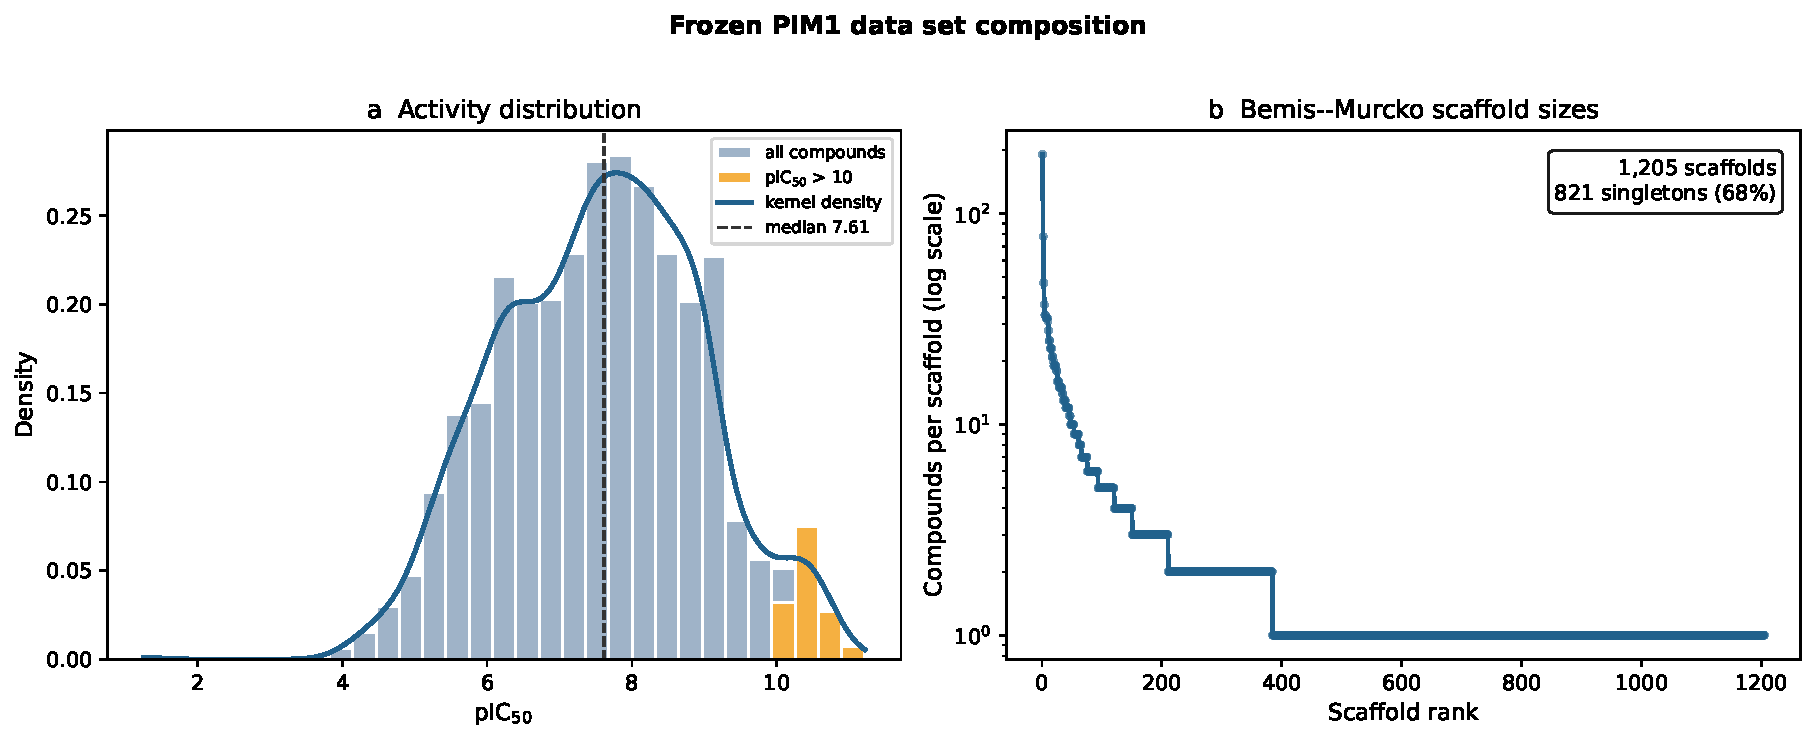
\includegraphics[width=\textwidth]{figs/fig1_dataset.pdf}
\caption{\textbf{Scope of the curated PIM1 dataset.}
(a) Distribution of pIC$_{50}$ across the 3,110 curated compounds (bars; kernel-density
overlay). The bulk lies between 4 and 10 (median 7.61, dashed line); 141 compounds have
pIC$_{50} > 10$ (nominal IC$_{50} < 100$ pM, amber). These values are retained and their
source-level provenance is described in the curation audit.
(b) Rank--size distribution of Bemis-Murcko scaffolds (log $y$-axis): 1,205 unique
scaffolds, of which 821 (68\%) are singletons, with the largest single class holding
191 compounds. Scaffold splitting keeps every member of a scaffold class on one side of
the train/test partition, so this diversity sets the difficulty of the prediction task.}
\label{fig:dataset}
\end{figure}

\subsection{Model Comparison}

Table~\ref{tab:model_comparison} summarizes the performance of all 11 models under
outer scaffold-group cross-validation with inner tuning and holdout evaluation.

\begin{table}[H]
\centering
\caption{Model performance under scaffold-based splitting.
         CV $R^2$ is the mean $\pm$ std of five outer-fold scores from the inner-tuned
         GroupKFold procedure.
         Holdout metrics are descriptive results for the 519-compound partition formed
         from 20\% of scaffold groups. The bold model was selected before holdout evaluation.}
\label{tab:model_comparison}
{\small
\setlength{\tabcolsep}{4pt}
\begin{tabular}{lcccc}
\toprule
\textbf{Model} & \textbf{CV $R^2$} & \textbf{Holdout $R^2$} & \textbf{Holdout RMSE} & \textbf{Holdout MAE} \\
\midrule
% Generated by generate_manuscript_artifacts.py; do not edit by hand.
\textbf{StackingEnsemble} & $0.700 \pm 0.015$ & 0.705 & 0.711 & 0.542 \\
VotingEnsemble & $0.690 \pm 0.018$ & 0.677 & 0.744 & 0.579 \\
Ridge & $0.683 \pm 0.015$ & 0.680 & 0.739 & 0.582 \\
RandomForest & $0.681 \pm 0.029$ & 0.694 & 0.723 & 0.537 \\
Lasso & $0.674 \pm 0.011$ & 0.660 & 0.763 & 0.600 \\
ElasticNet & $0.673 \pm 0.016$ & 0.681 & 0.739 & 0.582 \\
GradientBoosting & $0.661 \pm 0.026$ & 0.637 & 0.788 & 0.620 \\
KNeighbors & $0.659 \pm 0.044$ & 0.663 & 0.760 & 0.567 \\
LinearRegression & $0.658 \pm 0.023$ & 0.650 & 0.773 & 0.609 \\
AdaBoost & $0.501 \pm 0.077$ & 0.422 & 0.994 & 0.829 \\
DecisionTree & $0.477 \pm 0.032$ & 0.571 & 0.857 & 0.659 \\
%
\cr
\bottomrule
\end{tabular}
}
\end{table}

Under the prespecified rule, \SelectedModel{} had the highest mean outer-fold score
($R^2 = \SelectedCVRtwo{} \pm \SelectedCVRtwoSD{}$) and was therefore selected before
holdout evaluation. Its observed holdout performance was $R^2 = \SelectedHoldoutRtwo{}$,
RMSE $= \SelectedHoldoutRMSE{}$, and MAE $= \SelectedHoldoutMAE{}$ pIC$_{50}$ units.
The remaining models provide useful descriptive comparators (Table~\ref{tab:model_comparison}),
but one holdout partition and five outer folds do not establish a definitive ranking among
numerically close candidates.

\begin{figure}[t]
\centering
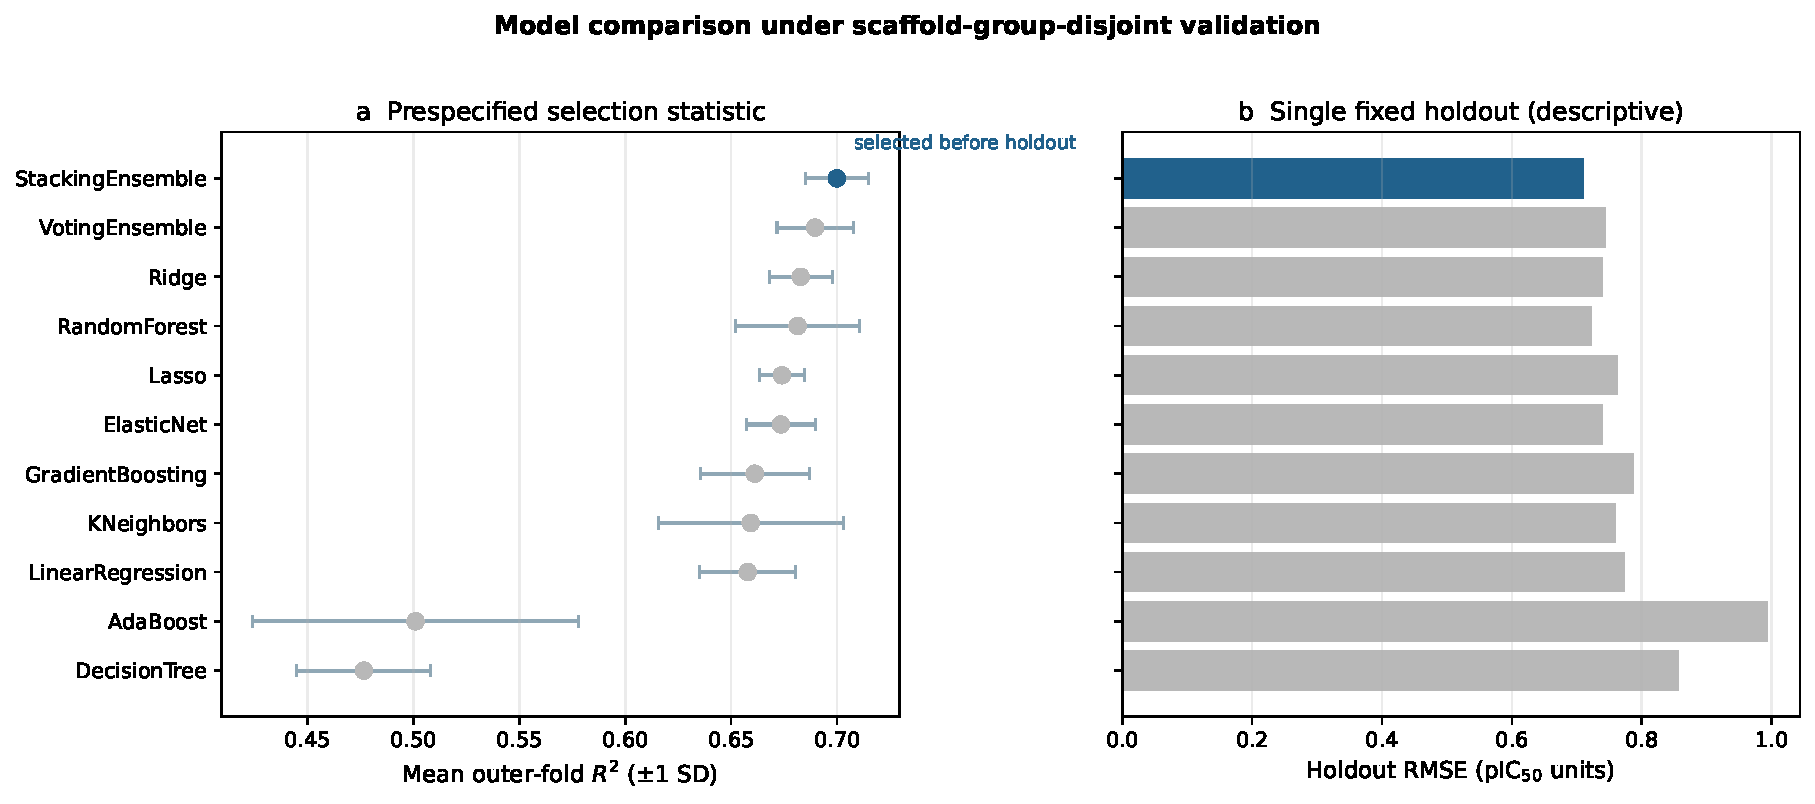
\includegraphics[width=\textwidth]{figs/fig2_model_comparison.pdf}
\caption{\textbf{Model comparison under scaffold-group-disjoint validation.}
(a) Mean outer-fold $R^2$ (point) with $\pm$1 SD error bars for all 11 models.
The highlighted \SelectedModel{} was selected by this quantity before holdout evaluation.
(b) RMSE on the single fixed holdout, displayed descriptively rather than as a model-selection
criterion. $n=\HoldoutCompounds{}$ compounds from \HoldoutScaffoldGroups{} scaffold groups.}
\label{fig:models}
\end{figure}

\begin{figure}[t]
\centering
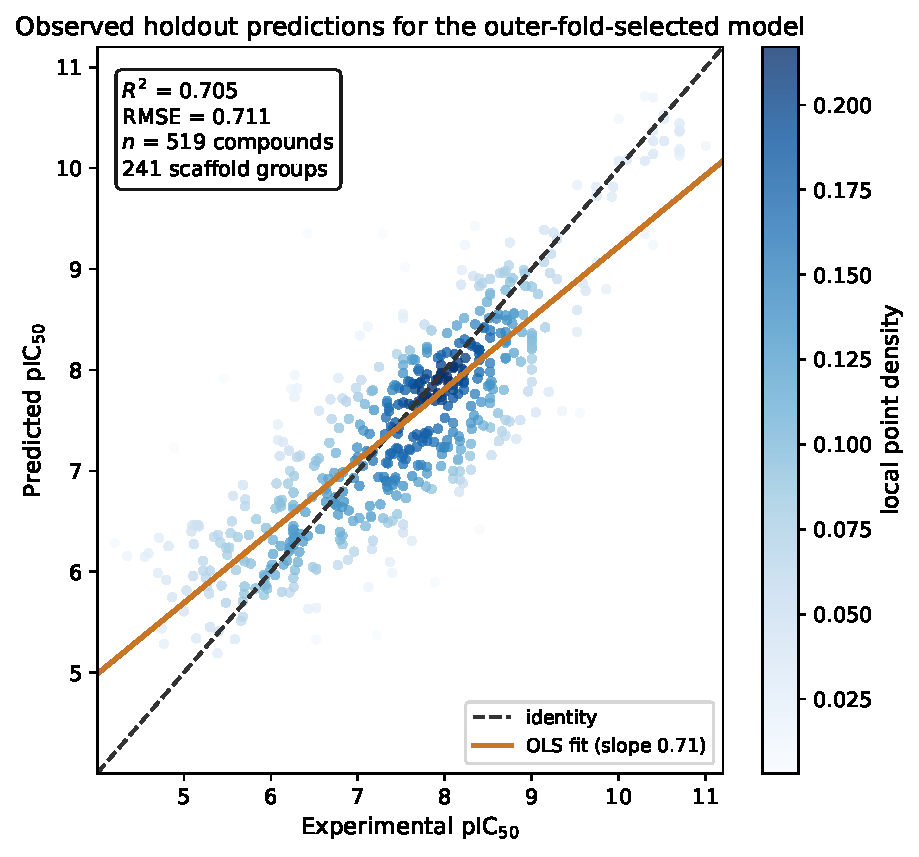
\includegraphics[width=0.62\textwidth]{figs/fig3_predictions.pdf}
\caption{\textbf{Predicted versus experimental pIC$_{50}$ for the outer-fold-selected
\SelectedModel{} on the scaffold-group holdout.} Points are the \HoldoutCompounds{} holdout compounds, shaded by local density;
the dashed line is the identity ($y = x$) and the solid line the ordinary-least-squares fit.
$R^2 = \SelectedHoldoutRtwo{}$, RMSE $= \SelectedHoldoutRMSE{}$ pIC$_{50}$ units.
The plot is a post-selection evaluation on one split.}
\label{fig:predictions}
\end{figure}

\enlargethispage{2\baselineskip}
Figure~\ref{fig:predictions} shows the \SelectedModel{} predictions for the fixed
scaffold-group holdout. The fitted line provides a descriptive view of calibration on this
partition; it is not a prospective validation analysis.

\subsection{Statistical Comparison}

Exploratory exact Wilcoxon signed-rank comparisons of the \SelectedModel{} outer-fold
scores against each alternative are reported in Table~\ref{tab:statistical}. With only five
paired folds, the smallest attainable two-sided exact $p$ value is 0.0625. Therefore a
non-significant result is not evidence of equivalence, and these comparisons are not used
to make a confirmatory superiority or tie claim.

\begin{table}[H]
\centering
\caption{Exploratory comparison of \SelectedModel{} against the alternatives using five
         paired outer-fold $R^2$ scores. $\Delta R^2$ is selected-model minus comparator;
         exact Wilcoxon $p$ values are descriptive because $n=5$ is underpowered.}
\label{tab:statistical}
{\small
\setlength{\tabcolsep}{4pt}
\begin{tabular}{lcccc}
\toprule
\textbf{Comparator} & \textbf{CV $R^2$} & \textbf{$\Delta R^2$} & \textbf{Wilcoxon $p$} & \textbf{Std. diff.} \\
\midrule
% Generated by generate_manuscript_artifacts.py; do not edit by hand.
VotingEnsemble & 0.690 & 0.010 & 0.0625 & 0.55 \\
Ridge & 0.683 & 0.017 & 0.0625 & 1.02 \\
RandomForest & 0.681 & 0.018 & 0.1250 & 0.71 \\
Lasso & 0.674 & 0.026 & 0.0625 & 1.79 \\
ElasticNet & 0.673 & 0.026 & 0.0625 & 1.51 \\
GradientBoosting & 0.661 & 0.039 & 0.0625 & 1.64 \\
KNeighbors & 0.659 & 0.041 & 0.0625 & 1.11 \\
LinearRegression & 0.658 & 0.042 & 0.0625 & 1.95 \\
AdaBoost & 0.501 & 0.199 & 0.0625 & 3.21 \\
DecisionTree & 0.477 & 0.223 & 0.0625 & 8.07 \\
%
\cr
\bottomrule
\end{tabular}
}
\end{table}

\enlargethispage{\baselineskip}
Compound-level bootstrap 95\% intervals (1,000 resamples) for the \SelectedModel{}
on the fixed holdout were $R^2 = \SelectedHoldoutRtwo{}$
[$\BootstrapRtwoLower{}, \BootstrapRtwoUpper{}$], RMSE $= \SelectedHoldoutRMSE{}$
[$\BootstrapRMSELower{}, \BootstrapRMSEUpper{}$], and MAE $= \SelectedHoldoutMAE{}$
[$\BootstrapMAELower{}, \BootstrapMAEUpper{}$]. These intervals characterize resampling
variation conditional on this partition, not variation across scaffold splits.

\subsection{Y-Randomization}

Across 30 label permutations, refits of the fixed \SelectedModel{} configuration gave
mean holdout $R^2 = \YRandomMean{} \pm \YRandomSD{}$, compared with
\SelectedHoldoutRtwo{} for the unpermuted labels. This negative control is consistent
with the fitted model using structure--activity signal in this frozen data set, but it
is not external validation.

\subsection{Applicability Domain}

The $k$-NN distance-based analysis classified \InDomainCount{} of \HoldoutCompounds{}
holdout compounds (\InDomainPercent{}\%) as in-domain. On this fixed partition, the
in-domain subset had $R^2 = \ADRtwoIn{}$ [\ADRtwoInLower{}, \ADRtwoInUpper{}] and RMSE
$= \ADRMSEIn{}$ [\ADRMSEInLower{}, \ADRMSEInUpper{}], compared with $R^2 = \ADRtwoOut{}$
[\ADRtwoOutLower{}, \ADRtwoOutUpper{}] and RMSE $= \ADRMSEOut{}$
[\ADRMSEOutLower{}, \ADRMSEOutUpper{}] for the \OutsideDomainCount{} outside-domain
compounds (Figure~\ref{fig:ad}). The small outside-domain subset and its conditional
bootstrap intervals warrant cautious interpretation; the analysis is a local reliability
diagnostic rather than proof of general predictive validity.

\begin{figure}[t]
\centering
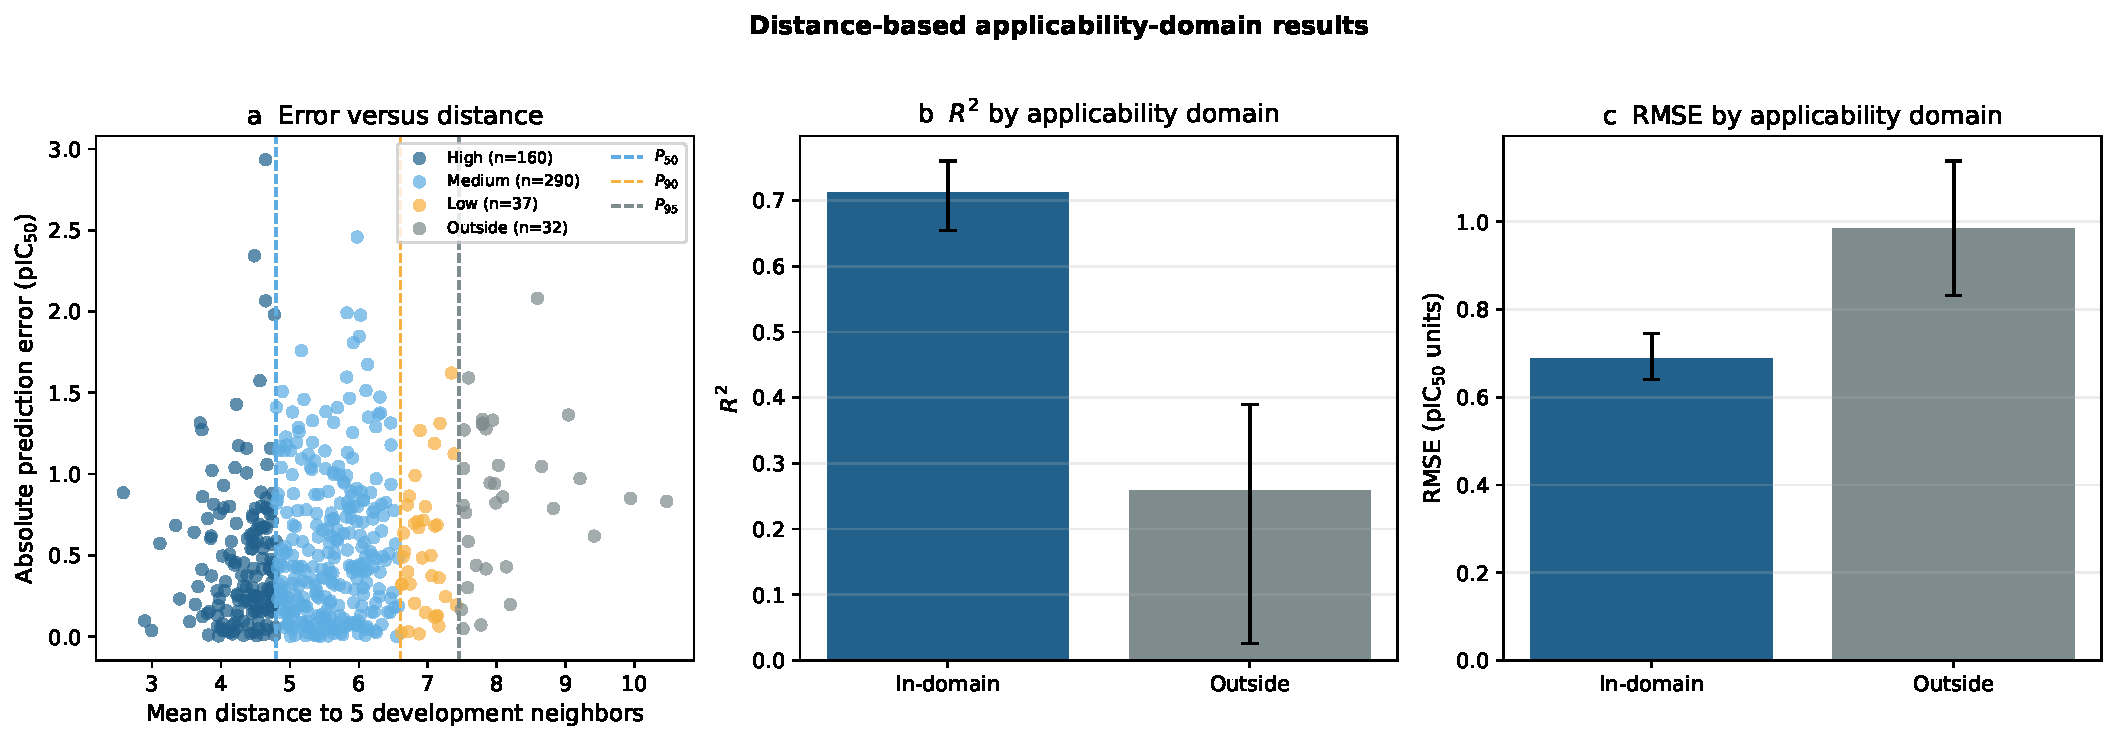
\includegraphics[width=\textwidth]{figs/fig4_applicability_domain.pdf}
\caption{\textbf{Distance-based applicability-domain results.}
(a) Absolute prediction error versus mean distance to five development neighbors, colored
by reliability category. Dashed lines mark $P_{50}$, $P_{90}$, and $P_{95}$ of development
distances (\ADMedianDistance{}, \ADNinetiethDistance{}, and \ADNinetyFifthDistance{}, respectively). (b--c) $R^2$ and RMSE inside
and outside the domain, with compound-bootstrap 95\% intervals. These outcomes are
conditional on one fixed holdout.}
\label{fig:ad}
\end{figure}

Per-scaffold error summaries are provided as an aid to inspecting which held-out chemical
series were difficult under this split. They do not identify a generalizable error mechanism.

\subsection{Model Interpretability}

\enlargethispage{\baselineskip}
Permutation importance for \SelectedModel{} ranks processed features by the loss of
holdout $R^2$ after a feature is shuffled (Figure~\ref{fig:interp}a). The result is
conditional on correlated features, this fitted model, and the fixed holdout. It therefore
describes model-specific feature associations rather than chemical or biological mechanisms.

Ridge coefficients in Figure~\ref{fig:interp}b come from a separately fitted Ridge
comparator, not from \SelectedModel{}. Their signs show conditional associations in that
comparator and should not be interpreted as the drivers of the selected model or of PIM1 potency.

\begin{figure}[t]
\centering
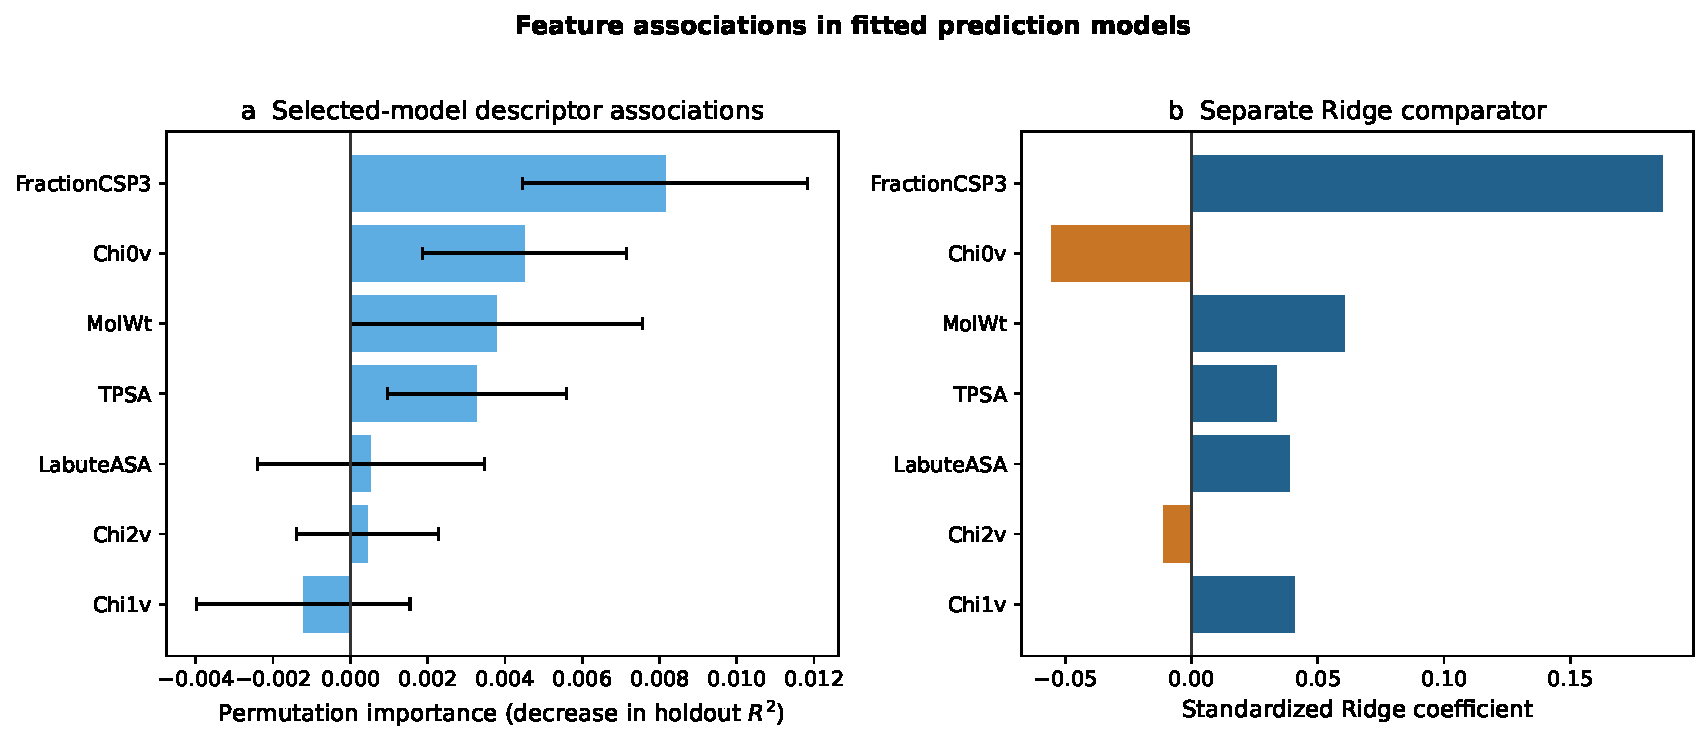
\includegraphics[width=\textwidth]{figs/fig5_interpretability.pdf}
\caption{\textbf{Feature associations in fitted prediction models, not mechanistic drivers.}
(a) Permutation importance for the \SelectedModel{} (decrease in holdout $R^2$ on feature
permutation; mean $\pm$ SD over 30 repeats) for retained physicochemical descriptors.
(b) Standardized coefficients of a separate Ridge comparator for the same descriptors.
Both panels are conditional, associative summaries of this data and split.}
\label{fig:interp}
\end{figure}

\section{Discussion}

\subsection{Performance in Context}

The observed holdout $R^2 = \SelectedHoldoutRtwo{}$ for \SelectedModel{} should be read as
an estimate conditional on one scaffold-group partition, rather than as a broadly established
benchmark rank for kinase QSAR.
\citet{martin2017profile} demonstrated across 159 kinase assays that single-task
Random Forest regression achieved a median $R^2_{\text{ext}}$ of only $\sim$0.12 under
realistic splitting conditions, and even multi-task approaches like pQSAR 2.0 reached
only $\sim$0.55 median $R^2_{\text{ext}}$.
This is not a like-for-like comparison, however: \citet{martin2017profile} report medians
across 159 diverse kinase assays under prospective-style evaluation, whereas our value is
for a single, data-rich target (PIM1) under a Bemis-Murcko scaffold split---a generally
different regime. It supplies context, not a direct performance comparison or a claim of
superiority.

\subsection{Experimental Uncertainty}

The RMSE of \SelectedHoldoutRMSE{} pIC$_{50}$ units corresponds to an approximately
$10^{\SelectedHoldoutRMSE{}}$-fold concentration error on this scale. Heterogeneous
IC$_{50}$ values aggregated from multiple laboratories and assay formats have substantial
experimental variability \citep{kramer2012experimental}, but this reference does not establish
an endpoint-specific PIM1 IC$_{50}$ noise floor for the present compilation. Replicate data
were not available to estimate that uncertainty directly.
Metrics such as $R^2$ can be misleading when the activity range is narrow
\citep{alexander2015beware}; we therefore report RMSE and MAE alongside $R^2$
following best practices for error metrics in QSAR \citep{roy2016some}.

\subsection{Model Representation}
\label{sec:representation}

Morgan fingerprints were reduced via PCA (95\% variance) for the linear and distance-based
models, primarily for computational efficiency and to provide a compact representation.
Because \citet{svetnik2003random} showed that tree ensembles handle high-dimensional sparse
fingerprints natively and can be harmed by PCA, the four standalone tree-based models
(Random Forest, Gradient Boosting, AdaBoost, Decision Tree) were instead trained on the raw
2048-bit fingerprints.
Under this representation-aware setup, the raw-fingerprint RandomForest can be compared
with the PCA-based models in Table~\ref{tab:model_comparison}. The one-split holdout values
and five-fold exploratory comparisons do not establish that any close pair is tied or that
one approach is generally superior.
We note one representation caveat in the ensemble meta-learners: the VotingEnsemble and
StackingEnsemble were fit on the PCA-reduced representation, so their Random Forest and
Gradient Boosting base learners---unlike their standalone counterparts---operated on PCA
components rather than raw bits.
Because the standalone raw-fingerprint RandomForest provides a strong individual-model
comparator in this run, giving each ensemble base learner its preferred representation
(for example, via per-estimator pipelines) is a natural refinement that may improve
ensemble performance.

\subsection{Limitations and Future Directions}

\textbf{Conditional validation.}
All reported performance estimates are conditional on one fixed scaffold-group holdout and
its particular chemical-series composition. The compound-bootstrap intervals do not quantify
variation across scaffold splits. Repeated seeded scaffold-group splits and a temporally
separated or independently generated external test set are needed to assess robustness and
transportability.

\textbf{Deep learning comparison.}
This study benchmarks 11 traditional machine learning algorithms but does not include
graph neural networks (GNNs) or deep learning models.
Recent work has demonstrated the potential of GNNs for molecular property prediction,
including the directed message-passing neural network (D-MPNN) of \citet{yang2019analyzing}
and various graph attention architectures.
\citet{tropsha2024integrating} defined ``deep QSAR'' as an emerging standard in the field.
Benchmarking GNNs against our ensemble approach on PIM1 data is a key future direction.

\textbf{External validation.}
The outer-fold procedure estimates the implemented tuning protocol, but the inner-fold
preprocessing limitation described in Methods remains, and \citet{gramatica2014external}
argues convincingly that ``CV should not be considered as external validation.''
A truly independent test set---from a different time period, laboratory, or database---would
substantially strengthen the generalizability claims.
Temporal splitting using ChEMBL deposition dates is a promising approach for future work.

\textbf{Biological framing.}
PIM1 has documented roles in PDAC biology, but PIM3 is the more prominently expressed
family member in pancreatic tumors \citep{li2006pim3}.
Our computational models predict PIM1 inhibitory potency and should be understood as
tools for prioritizing chemical matter with predicted PIM1 activity, with potential
relevance to PDAC given PIM1's reported biological roles rather than as direct PDAC
drug candidates. No PIM-family selectivity, cellular efficacy, ADMET property, or prospective
experimental validation was evaluated.

\textbf{Data currency.}
The dataset was drawn from ChEMBL v33 (May 2023).
While subsequent releases may contain additional PIM1 data, the dataset was locked for
reproducibility.

\section{Conclusions}

We present a scaffold-aware QSAR study of PIM1 kinase inhibitors that combines
ECFP6 fingerprints with physicochemical descriptors under scaffold-group-disjoint evaluation.
The outer-fold-selected \SelectedModel{} obtained holdout $R^2 = \SelectedHoldoutRtwo{}$
and RMSE $= \SelectedHoldoutRMSE{}$ pIC$_{50}$ units on the fixed 519-compound partition.
The curation audit, label-randomization control, distance-based applicability domain,
associative feature analyses, exploratory fold comparisons, and bootstrap intervals make the
scope of this benchmark transparent. They do not replace repeated-split, temporal, external,
or experimental validation. The models and analysis pipeline are implemented in open-source
Python using scikit-learn and RDKit.

\section*{Data and Code Availability}

The frozen input files, source code, generated result tables, and SHA-256 checksums used
for this manuscript are available in the project's
\href{https://github.com/MikeZenko/Scaffold-Aware-QSAR-Modeling-PIM1}{GitHub repository}. The curation audit is
stored in \texttt{results/CHEMBL2147/data\_curation\_audit.json}; the selected-model record,
split manifest, and generated manuscript metrics are stored alongside the other results.
Because the acquisition script queries the live ChEMBL REST API, reproduction of this manuscript
should start from the archived frozen inputs and their checksums, not from a fresh live download.
The exact Python package versions are recorded in \texttt{requirements.txt} and
\texttt{environment.yml}.

\begin{thebibliography}{99}

\bibitem[Abdelaziz et~al.(2017)]{abdelaziz2017}
Abdelaziz, A. et~al. (2017).
3D-QSAR study of PIM1 kinase inhibitors using CoMFA and CoMSIA approaches.
\textit{Journal of Molecular Structure}, 1130, 119--129.

\bibitem[Alexander et~al.(2015)]{alexander2015beware}
Alexander, D.~L.~J., Tropsha, A., \& Winkler, D.~A. (2015).
Beware of $R^2$: Simple, unambiguous assessment of the prediction accuracy of QSAR and QSPR models.
\textit{Journal of Chemical Information and Modeling}, 55(7), 1316--1322.

\bibitem[Almukadi et~al.(2023)]{almukadi2023}
Almukadi, H. et~al. (2023).
Machine learning classification of PIM1 kinase inhibitors.
\textit{Frontiers in Chemistry}, 11, 1162087.

\bibitem[Bemis \& Murcko(1996)]{bemis1996properties}
Bemis, G.~W. \& Murcko, M.~A. (1996).
The properties of known drugs. 1. Molecular frameworks.
\textit{Journal of Medicinal Chemistry}, 39(15), 2887--2893.

\bibitem[Breiman(2001)]{breiman2001random}
Breiman, L. (2001).
Random forests.
\textit{Machine Learning}, 45(1), 5--32.

\bibitem[Chen et~al.(2008)]{chen2008pim1}
Chen, J. et~al. (2008).
Pim-1 plays a pivotal role in hypoxia-induced chemoresistance.
\textit{Cancer Biology \& Therapy}, 7(4), 555--564.

\bibitem[Cherkasov et~al.(2014)]{cherkasov2014qsar}
Cherkasov, A. et~al. (2014).
QSAR modeling: where have you been? Where are you going to?
\textit{Journal of Medicinal Chemistry}, 57(12), 4977--5010.

\bibitem[Gramatica(2014)]{gramatica2014external}
Gramatica, P. (2014).
External evaluation of QSAR models, in addition to cross-validation: verification of predictive capability on totally new chemicals.
\textit{Molecular Informatics}, 33(4), 311--314.

\bibitem[Kr\"amer et~al.(2012)]{kramer2012experimental}
Kr\"amer, C. et~al. (2012).
The experimental uncertainty of heterogeneous public $K_i$ data.
\textit{Journal of Medicinal Chemistry}, 55(11), 5165--5173.

\bibitem[Li et~al.(2006)]{li2006pim3}
Li, Y.~Y. et~al. (2006).
Pim-3, a proto-oncogene with serine/threonine kinase activity, is aberrantly expressed in human pancreatic cancer and phosphorylates Bad to block Bad-mediated apoptosis in human pancreatic cancer cell lines.
\textit{Cancer Research}, 66(13), 6741--6747.

\bibitem[Martin et~al.(2017)]{martin2017profile}
Martin, E.~J. et~al. (2017).
Profile-QSAR 2.0: Kinase virtual screening accuracy comparable to four-concentration IC$_{50}$s for realistically novel compounds.
\textit{Journal of Chemical Information and Modeling}, 57(8), 2077--2088.

\bibitem[Svetnik et~al.(2003)]{svetnik2003random}
Svetnik, V., Liaw, A., Tong, C., Culberson, J.~C., Sheridan, R.~P., \& Feuston, B.~P. (2003).
Random forest: A classification and regression tool for compound classification and QSAR modeling.
\textit{Journal of Chemical Information and Computer Sciences}, 43(6), 1947--1958.

\bibitem[Nadeau \& Bengio(2003)]{nadeau2003inference}
Nadeau, C. \& Bengio, Y. (2003).
Inference for the generalization error.
\textit{Machine Learning}, 52(3), 239--281.

\bibitem[OECD(2007)]{oecd2007guidance}
OECD (2007).
Guidance document on the validation of (quantitative) structure-activity relationship [(Q)SAR] models.
\textit{OECD Environment Health and Safety Publications, Series on Testing and Assessment}, No.~69.

\bibitem[R\'acz et~al.(2022)]{racz2022combination}
R\'acz, A. et~al. (2022).
Effect of dataset size and train/test split ratios in QSAR/QSPR---multiclass classification.
\textit{Frontiers in Chemistry}, 9, 830365.

\bibitem[Rahib et~al.(2014)]{rahib2014projecting}
Rahib, L. et~al. (2014).
Projecting cancer incidence and deaths to 2030: the unexpected burden of thyroid, liver, and pancreas cancers in the United States.
\textit{Cancer Research}, 74(11), 2913--2921.

\bibitem[Rodr\'iguez-P\'erez \& Bajorath(2020)]{rodriguezperez2020interpretation}
Rodr\'iguez-P\'erez, R. \& Bajorath, J. (2020).
Interpretation of machine learning models using Shapley values: application to compound potency and multi-target activity predictions.
\textit{Journal of Computer-Aided Molecular Design}, 34(10), 1013--1026.

\bibitem[Rogers \& Hahn(2010)]{rogers2010extended}
Rogers, D. \& Hahn, M. (2010).
Extended-connectivity fingerprints.
\textit{Journal of Chemical Information and Modeling}, 50(5), 742--754.

\bibitem[Roy et~al.(2016)]{roy2016some}
Roy, K. et~al. (2016).
Some case studies on application of ``$r_m^2$'' metrics for judging quality of quantitative structure-activity relationship predictions: emphasis on scaling of response data.
\textit{Journal of Computational Chemistry}, 37(18), 1507--1515.

\bibitem[Siegel et~al.(2025)]{siegel2025cancer}
Siegel, R.~L. et~al. (2025).
Cancer statistics, 2025.
\textit{CA: A Cancer Journal for Clinicians}, 75(1), 10--33.

\bibitem[Tropsha et~al.(2024)]{tropsha2024integrating}
Tropsha, A., Isayev, O., Varnek, A., Schneider, G., \& Cherkasov, A. (2024).
Integrating QSAR modelling and deep learning in drug discovery: the emergence of deep QSAR.
\textit{Nature Reviews Drug Discovery}, 23(2), 141--155.

\bibitem[Wu et~al.(2018)]{wu2018moleculenet}
Wu, Z. et~al. (2018).
MoleculeNet: a benchmark for molecular machine learning.
\textit{Chemical Science}, 9(2), 513--530.

\bibitem[Xu et~al.(2011)]{xu2011pim1}
Xu, D. et~al. (2011).
The oncogenic kinase Pim-1 is modulated by K-Ras signaling and mediates transformed growth and radioresistance in human pancreatic ductal adenocarcinoma cells.
\textit{Carcinogenesis}, 32(4), 488--495.

\bibitem[Yang et~al.(2019)]{yang2019analyzing}
Yang, K. et~al. (2019).
Analyzing learned molecular representations for property prediction.
\textit{Journal of Chemical Information and Modeling}, 59(8), 3370--3388.

\bibitem[Zdrazil et~al.(2024)]{zdrazil2024chembl}
Zdrazil, B. et~al. (2024).
The ChEMBL Database in 2024: a drug discovery platform spanning genomics, chemical biology and clinical data.
\textit{Nucleic Acids Research}, 52(D1), D1180--D1192.

\end{thebibliography}

\end{document}
